%*****************************************
\chapter{Geospatial assessment of phosphorus recovery through the deployment of struvite precipitation systems}\label{ch:Struvite}
\chaptermark{Geospatial assessment of P recovery by struvite precipitation}
%*****************************************
\section*{Abstract}
Nutrient pollution is one of the major worldwide water quality problems, resulting in environmental and public health issues. Agricultural activities are the main source of nutrient release emissions, and the livestock industry has been proven to be directly related to the presence of high concentrations of phosphorus in the soil, which potentially can reach waterbodies by runoff. To mitigate the phosphorus pollution of aquatic systems, the implementation of nutrient recovery processes allows the capture of phosphorus, preventing its release into the environment. Particularly, the use of struvite precipitation produces a phosphorus-based mineral that is easy to transport, enabling redistribution of phosphorus to deficient locations. However, livestock leachate presents some characteristics that hinder struvite precipitation, preventing extrapolation of the results obtained from wastewater studies to cattle waste. Consideration of these elements is essential to determine the optimal operating conditions for struvite formation, and for predicting the amount of struvite recovered. In this work, a detailed thermodynamic model for precipitates formation from cattle waste is used to develop surrogate models to predict the formation of struvite and calcium precipitates from cattle waste. The variability in the organic waste composition, and how it affects the production of struvite, is captured through a probability framework based on the Monte Carlo method embedded in the model. Consistent with the developed surrogate models, the potential of struvite production to reduce the phosphorus releases from the cattle industry to watersheds in the United States has been assessed. Also, the more vulnerable locations to nutrient pollution were determined using the techno-ecological synergy sustainability metric (TES) by evaluating the spatial distribution and balance of phosphorus from agricultural activities. Although only struvite formation from cattle operations is considered, reductions between 22\% and 36\% of the total phosphorus releases from the agricultural sector, including manure releases and fertilizer application, can be achieved.

%\smallskip
Keywords: Organic waste; Phosphorus; Nutrient pollution; Struvite; Thermodynamics

\newpage

\section*{Resumen}
La contaminación por nutrientes es uno de los principales problemas de calidad del agua en todo el mundo, lo que provoca problemas medioambientales y de salud pública. Las actividades agrícolas son la principal fuente de emisión de nutrientes, y se ha demostrado que la industria ganadera está directamente relacionada con la presencia de altas concentraciones de fósforo en el suelo, que potencialmente pueden llegar a las masas de agua por escorrentía. Para mitigar la contaminación por fósforo de los sistemas acuáticos, la implementación de procesos de recuperación de nutrientes permite la captura de fósforo, evitando su liberación al medio ambiente. En particular, el uso de la precipitación de estruvita produce un mineral a base de fósforo que es fácil de transportar, lo que permite la redistribución del fósforo a lugares deficientes. Sin embargo, los lixiviados ganaderos presentan algunas características que dificultan la precipitación de estruvita, impidiendo la extrapolación de los resultados obtenidos en los estudios de aguas residuales a los residuos ganaderos. La consideración de estos elementos es esencial para determinar las condiciones óptimas de operación para la formación de estruvita, y para predecir la cantidad de estruvita recuperada. En este trabajo, se utiliza un modelo termodinámico detallado para la formación de precipitados a partir de residuos ganaderos con el fin de desarrollar modelos sustitutos para predecir la formación de estruvita y precipitados de calcio a partir de residuos ganaderos. La variabilidad en la composición de los residuos orgánicos, y cómo afecta a la producción de estruvita, se capta a través de un marco probabilístico basado en el método de Monte Carlo integrado en el modelo. En consonancia con los modelos sustitutos desarrollados, se ha evaluado el potencial de la producción de estruvita para reducir las emisiones de fósforo de la industria ganadera a las cuencas hidrográficas de Estados Unidos. Asimismo, se determinaron los lugares más vulnerables a la contaminación por nutrientes utilizando la métrica de sostenibilidad de la sinergia tecno-ecológica (TES) mediante la evaluación de la distribución espacial y el equilibrio del fósforo procedente de las actividades agrícolas. Aunque sólo se tiene en cuenta la formación de estruvita procedente de las explotaciones ganaderas, se pueden conseguir reducciones de entre el 22\% y el 36\% del total de las emisiones de fósforo procedentes del sector agrícola, incluidas las emisiones de estiércol y la aplicación de fertilizantes.

\medskip
Palabras clave: Residuos orgánicos; Fósforo; Contaminación por nutrientes; Estruvita; Termodinámica

\newpage

\begin{refsection}[referencesCh3]
\section{Introduction}
Livestock farming and other agricultural activities have altered the natural nutrient cycles. Phosphorus, one of the three plant-grow macronutrients, enters to the global cycle as phosphate rock, which through erosion and chemical weathering is transferred to soils and waterbodies. Also, phosphorus deposited in soils will reach fresh and marine waterbodies by runoff. Phosphorus in rivers is transported to stagnant waterbodies (such as lakes) and oceans, reaching the bottom of lakes and oceans as sediments. The cycle is closed when the buried phosphorus is uplifted again by tectonic processes. Along the cycle, phosphorus can be taken by plants and algae, but after the death of living organisms it returns to the cycle \citep{RUTTENBERG2001401}. This global natural cycle is largely altered by human activities through the mining and shipping of phosphate rock, mainly for fertilizer production, resulting in unbalanced phosphorus releases to the environment.

Nutrient pollution from anthropogenic sources has become as a critical worldwide water quality problems. Nutrient contamination results in environmental and public health issues as a result of the exponential growth of algae, cyanobacteria, and the occurrence of harmful algal blooms (HABs), which turns into dead zones and hypoxia due to the aerobic degradation of the algal biomass by bacteria; shifting the distribution of aquatic species and releasing toxins in drinking water \citep{Sampat2}. In addition, the development of HABs and eutrophication processes contributes to climate change through the emission of large amounts of strong greenhouse gases such as $\text{CH}_{4}$ and $\text{N}_{2}\text{O}$ \citep{Beaulieu}.

However, phosphorus is a limited non-renewable resource, essential nutrient to support life, and widely used as fertilizer to increase crop yields. Actually, phosphorus is one of the most sensitive elements to depletion, as it is a key agricultural fertilizer that has no known substitute. Current global reserves of phosphate rock could be depleted in the next 50 to 100 years \citep{Cordell}. Therefore, the development of a circular economy around phosphorus capable of recovering the nutrient and reintegrating it into the productive cycle is not only desirable but also a necessary measure to reach sustainable development. Agricultural activities are the main source of nutrients in waterbodies \citep{Dzombak}, and among them, livestock industry is one of the largest economic sectors. Additionally, the increasing income-spending potential of the middle class in developing countries has increased the demand for dairy and beef products, resulting in the generation of large amounts of livestock organic waste. Considering that an average dairy cow generates 51.19 kg of raw manure per day \citep{USDAWaste}, the total phosphorus excreted is 11.02 kg per year per animal, equivalent to 5.96 kg of phosphorus as phosphate per year per animal. In the U.S. as of January 2020, a total of 94.4 million head has been reported \citep{USDACattle2020}. Thus, this shows potential phosphate U.S. releases of $562.6\cdot10^{6}$ kg/yr. \citet{Sampat} presented the link between the presence of livestock facilities and larger concentrations of phosphorus in soil, which potentially can be lost as runoff reaching waterbodies. 
For animals on pasture, organic waste should not be a resource of concern if stocking rates are not excessive. However, for concentrate animal feeding operations (CAFOs), manure should be correctly managed due to the high rates and spatial concentration of the organic waste generated, representing potential environmental issues. Usually, manure is collected in the animal living zones, and stored as liquid or slurry to be further spread in croplands as nutrient supplementation; or as solid in dry stacking or composting facilities to be sold as compost. Liquid fraction of manure can be also treated in aerobic or anaerobic ponds. However, these approaches do not allow a correct nutrient management since nutrients concentration is variable and not well defined, and nitrogen and phosphorus are unbalanced regarding the nutrient necessities of plans, i.e., if nitrogen demand is covered, there is a surplus in the phosphorus supply which can runoff to waterbodies, and if phosphorus demand is covered, there is a deficit in the nitrogen supply, being necessary to apply additional fertilizers. In addition, during rainy periods the applied manure can runoff, dragging the nutrients contained in it. Nonetheless, phosphorus from liquid cattle waste, either processed in an anaerobic digestion stage or raw waste, can be potentially recovered through different processes \citep{muhmood2019formation}, reducing the nutrient inputs to waterbodies and its consequential environmental, economic, and social impacts. Among these, it is found that struvite production is one of the most promising cost-effective choices for the recovery of nutrients from cattle waste \citep{Martin}. Struvite is a phosphate-based mineral, which can be applied as a slow release fertilizer \citep{Richards}, allowing the redistribution of phosphorus from livestock facilities to nutrient-deficient locations.

Previous studies report struvite formation from different sources of waste, such as municipal wastewater treatment plants \citep{Battistoni}, mineral fertilizer industry \citep{Matynia}, or agricultural industry \citep{Shashvatt}. Thermodynamic models representing the formation of struvite and other precipitates have been also developed for various wastes including liquid swine manure \citep{celen_using_2007}, human urine \citep{Harada, ronteltap_struvite_2007}, and municipal wastewater \citep{rahaman_modeling_2014}. Additionally, some complex approaches considering the hydrodynamic and kinetic effects in the formation of struvite have been studied but limited to wastewater treatment \citep{rahaman_modeling_2014, mangin2004fluid}. However, the results obtained from those studies cannot be extrapolated to struvite formation from cattle organic waste, since these residues have some characteristics that hinder struvite formation, including high ionic strength, which reduces the effective concentration of ions; the presence of calcium ions competing for phosphate ions \citep{Yan}, which inhibits a selective recovery by nutrient precipitation techniques; and the high variability in the manure composition, as a function of the geographical area, the animal feed, etc. \citep{Tao}. Other controlling factors are the pH level, the magnesium-phosphorus ratio, and the alkalinity of the leachate. Therefore, for an accurate prediction of struvite formation from this waste, it is necessary to include within the thermodynamic model structure for precipitates formation the specific features  of cattle waste described above.

In this work, specific surrogate models to predict the production of struvite and calcium precipitates from cattle leachate are developed based on a detailed and robust thermodynamic model. In addition, the variability in the organic waste composition is captured through a probability framework based on Monte Carlo method. The reduced models obtained are used to evaluate the potential of struvite production from cattle waste to mitigate phosphorus releases in watersheds of the United States. Future applications of the developed surrogate models include the development of applications for environmental assessment and the design of policies to prevent nutrient releases, among others.

\section{Methods}
\subsection{Spatial resolution}
A watershed is an area of land which drains all the streams and rainfall to a common drainage, defining the spatial boundaries for the collection of lost elements as runoff. The surface  water  drainages of the U.S. are identified by the U.S. Geological Survey through the Hydrologic Unit Code system (HUC). The HUC system is a hierarchical system indicated by the number of digits in groups of two, with six levels identified by codes from 2 to 12 digits (i.e., HUC2 to HUC12). These levels refer to regions, subregions, basins, subbasins, watersheds, and subwatersheds. The spatial resolution of this study is the continental United States at watershed scale, considering the boundaries defined by the Hydrologic Unit Code system at 8 digits (HUC8), representing the subbasin level \citep{HUC8}.

\subsection{Assessment of anthropogenic phosphorus from agricultural activities}
\subsubsection{Phosphorus releases} \label{Preleases}
Agricultural emissions are one of the main sources of anthropogenic P releases due to the excessive use of commercial fertilizers and livestock manure for cropland nutrients needs and the uncontrolled nutrient runoff to waterbodies, although for some areas urban source releases can contribute significantly to the total P releases to the environment. However, this analysis is limited to the evaluation of phosphorus releases from agricultural activities \citep{Dzombak, Alexander_2008, SPARROW_report_1999}.

Watershed phosphorus releases $\left(E_{x}\right)$ are computed as the sum of the phosphorus releases from fertilizer applications to croplands and from the manure generated by livestock facilities. The releases of phosphorus to each watershed by manure emissions, accounting cattle, swine and poultry, and by fertilizers application, is reported by the IPNI NuGIS project. This is consitent with the most recent data available (year 2014) for fertilizers sales provided by the Association of American Plant Food Control Officials (AAPFCO), fitting the data to HUC8 watershed boundaries. More information about the methodology used for the estimation of agricultural phosphorus releases can be found in \citep{NuGIS}. Phosphorus content for several commercial phosphate fertilizers and different manure types can be found in \citet{OSU2017} and \citet{OSU2005} respectively.

\subsubsection{Phosphorus uptakes}
The elements considered for phosphorus uptake are the crops sown and managed by humans in each watershed. Additionally, the phosphorus retained by wetlands has been considered in the phosphorus balance. The phosphorus uptake by each type of vegetation at watershed level is computed as the product of the land area occupied, the grow yields per area unit and the phosphorus uptake per plant mass unit. Therefore, the total watershed phosphorus uptake $\left(U_{x}\right)$ is computed as the sum of the phosphorus uptake by each type of plant, Eq. \ref{eq:U_x}.

\begin{align}
%& U_{i} = \text{Area}_{i} \cdot \text{Yield}_{i} \cdot \text{P}_{\text{uptake }i} \ \forall \ i \ \in \ {\text{Plant varieties}} \label{eq:U_i} \\
& U_{x} = \sum^{i} \text{Area}_{i} \cdot \text{Yield}_{i} \cdot \text{P}_{\text{uptake }i} \ \forall \ i \ \in \ {\text{Plant varieties}} \label{eq:U_x}
\end{align}
Since different crops have different phosphorus uptakes and yield rates, the amount of each type of crop is estimated for each watershed. To determine the land cover uses, accounting croplands, pasturelands, wetlands and developed areas (urban areas), information available for the most recent year (2011) from the U.S. Environmental Protection Agency's (U.S. EPA) EnviroAtlas database is used \citep{EnviroAtlas}. Data from EnviroAtlas is provided with higher spatial resolution, at HUC12 level. To ensure spatial consistency, the data is reconciled at HUC8 level. Once the land uses of each watershed are known, data from the 2017 U.S. Census of Agriculture is used to determine the distribution of crops on croplands, considering corn, soybeans, small grains, cotton, rice, vegetables, orchards, greenhouse and other crops (namely oil crops, sugar crops, and fruits) \citep{2017CensusofAgriculture}. The data provided by the U.S. Census of Agriculture have a spatial resolution of HUC6. Therefore, it is reconciled at HUC8 level scaling by the area fraction represented by each HUC8 watershed over the total HUC6 hydrologic unit. If two or more crops were harvested from the same land during the year (double cropping), the area was counted for each crop. To determine the nutrients uptake of each type of crop, data from the U.S. Department of Agriculture (USDA) Waste Management field Handbook is considered  \citep{USDAWaste}. For croplands, the specific nutrient uptake values are used for corn, soybeans, cotton, rice and orchards, while average values including the most representative species are used for small grains, vegetables, greenhouse crops, pasture crops, and forest. For pasture lands the average nutrient uptake and crop yield including the main pasture crops: alfalfa, switchgrass and wheatgrass; for forests lands the nutrient uptake and crop yield of Northern hardwoods is considered, and for developed areas null nutrient uptake is considered. The wetlands phosphorus uptake value considered is 0.77 gP m$^{-2}$ year$^{-1}$, based in the data reported by \citet{Kadlec}.

\subsubsection{Phosphorus balance}
To reach environmental sustainability of a productive activity, the releases of phosphorus should be balanced with the phosphorus uptakes from that activity, reducing the impact over the original ecosystems as much as possible. To evaluate the balance of phosphorus releases involved in agricultural activities throughout the U.S. watersheds, the techno-ecological synergy (TES) sustainability metric proposed by \citet{TESmetric} has been considered, Eq. \ref{eq:TES}. A negative value of $V_{x}$ indicates that the emissions, $\left(E_{x}\right)$, are larger than the uptake capacity of the agricultural activities, $\left(U_{x}\right)$, impacting the ecosystems, while positive values reflect that the releases are lower than the uptake capacity.

\begin{align}
& V_{x} =\frac{\left(U_{x} - E_{x}\right)}{E_{x}} \label{eq:TES}
\end{align}

\subsection{Thermodynamic model for precipitates formation} \label{thermo_model}
The behavior of cattle leachate system has been evaluated through a thermodynamic model, evaluating the formation of different precipitates through chemical equilibrium and material balances, capturing the mutual dependencies based on the competition for the same ions. Four aqueous chemical systems have been considered, water, ammonium, phosphoric acid, and carbonates systems. Moreover, the formation of seven possible precipitates is evaluated: struvite, K-struvite, magnesium hydroxide, calcium hydroxide, calcium carbonate, hydroxyapatite, dicalcium phosphate, and tricalcium phosphate.

\subsubsection{Uncertainty in livestock organic waste composition} \label{comp_dist}
The variability in the composition of raw material creates operational difficulties that any material recovery process must deal with. The composition of cattle organic waste depends on multiple factors, among which are livestock feed, geographical area, climate, and other local factors of the livestock operation \citep{Tao}. Several elements of cattle manure composition play an active role in the formation of struvite and other precipitates. These include the high ionic strength, which reduces the effective concentration of ions; and the distribution ratios between calcium, ammonia and phosphate; and the leachate alkalinity, affecting the chemical equilibrium. To capture the uncertainty generated by the variability in the composition of cattle leachate, 37 data sets of 20 literature references containing the mass fraction of different elements comprising organic livestock waste are evaluated. To estimate feasible cattle leachate compositions, the probability density distribution of each element is calculated by fitting it to the kernel density estimate (KDEs). The selected probability density distributions are normal distribution, as shown in Eq. \ref{eq:normal_dist}, for the distribution of nitrogen, nitrogen as ammonia/total nitrogen ratio, and phosphorus; and lognormal distribution, as defined by  Eq. \ref{eq:lognormal_dist}, for phosphorus as phosphate/total phosphorus ratio, calcium, and potassium. The probability density distribution parameters for each evaluated compound are collected in Table \ref{table:PDD_paramenters}, where $\sigma$ is the standard deviation, $\sigma^2$ is the variance, $\mu$ is the mean of the distribution, $M$ is equal to $e^{\mu}$, and $\gamma$ is a displacement parameter. Kernel density estimations and probability density distributions for each element evaluated can be found in the Supplementary Material. 

The uncertainty in the composition of cattle waste is addressed through the evaluation of the thermodynamic model described in the following sections for multiple cattle waste compositions generated including the probability density distribution of each elements in a Monte Carlo model \citep{Thomopoulos}.

\begin{align}
f(x) = \frac{1}{\sqrt{2 \pi \sigma}}e^{- \frac{\left( x - \mu \right)^{2}}{2 \sigma ^ {2}}} & \label{eq:normal_dist} \\
f(x) = \frac{\frac{1}{\frac{x- \gamma}{M} \sigma \sqrt{2 \pi}} e^{-\frac{ln\left( \frac{x- \gamma}{M} \right)^{2}}{2 \sigma^{2}}}}{M} \label{eq:lognormal_dist}
\end{align}

\begin{table}[h] 
	\centering
	\caption{Probability density distributions parameters for cattle organic waste elements.} \label{table:PDD_paramenters}
	\resizebox{\columnwidth}{!}{
	\begin{tabular}{c c c c c c c c} %llrll
		\toprule
		\multicolumn{1}{c}{Param.}&\multicolumn{3}{c}{Normal distribution}&\multicolumn{1}{c}{Param.}&\multicolumn{3}{c}{Lognormal distribution} \\ \cmidrule(lr){2-4}\cmidrule(lr){6-8}%\hline 
		\\[-1em]
		&N		&$\text{N-NH}^{+}_{4}:\text{N}_{\text{total}}$		&P	&		&$\text{P-PO}_{4}^{3-}:\text{P}_{\text{total}}$		&$\text{Ca}$		&$\text{K}$ 		\\ \midrule
		$\mu$		&0.3841			&0.6200			&0.04000	&$M$		&42.15		&0.08000	&0.2600			\\ 
		$\sigma$	&0.1309			&0.1250			&0.03684	&$\sigma$		&0.0040		&0.4500		&0.8000		\\ 
		&				&				&			&$\gamma$		&-41.53		&0.04044	&0.03389		\\ 
		\bottomrule
	\end{tabular}
	}
\end{table}

\subsubsection{Initial conditions} \label{Initial parameters}
A set of initial conditions must be defined to establish the physico-chemical characteristics of the livestock organic material \citep{Tao}, see Table \ref{table:init_cond}. Please note that pH refers the adjusted pH for optimal struvite precipitation \citep{Tao, Zeng}. 

\begin{table}[h]
	\centering
	\caption{Initial conditions of the livestock organic material system} \label{table:init_cond}
	\resizebox{\columnwidth}{!}{
	\begin{tabular}{@{}ccc@{}}
		\toprule
		Variable               & Value                                                                                      & Unit                               \\ \midrule
		Temperature             & 298                                                                                        & K                                  \\
		pH                      & 9                                                                                          & -                                  \\
		Electrical conductivity ($EC$) & 18,800                                                                                     & $\frac{\mu \text{S}}{\text{cm}}$\\
		Alkalinity              & 3000-14500                                                                                 & mg of CaCO$_{3}$                        \\
		{[Ca$^{2+}$]}               & \begin{tabular}[c]{@{}c@{}} 0.075-0.175 \\ (determined by Monte Carlo model) \end{tabular}											& \% wt wet                          \\
		{[K$^{+}$]}                       & \begin{tabular}[c]{@{}c@{}} 0.10-0.65 \\ (determined by Monte Carlo model) \end{tabular}     & \% wt wet                          \\
		{[P-PO$_{4}^{3-}$]}                      & \begin{tabular}[c]{@{}c@{}} 0.001-0.024 \\ (determined by Monte Carlo model) \end{tabular} & \% wt wet                          \\
		{[N-NH$_{4}^{+}$]}                      & \begin{tabular}[c]{@{}c@{}} 0.015-0.64 \\ (determined by Monte Carlo model) \end{tabular}  & \% wt wet                          \\
		{[Mg$^{2+}$]}                      &  0-10                                                                                       &$\text{Mg}^{2+}/\text{PO}_{4}^{3-}$ molar ratio           \\ \bottomrule
	\end{tabular}
	}
\end{table}

\subsubsection{Activities} \label{Activity coefficients}
Since the cattle waste is a highly non-ideal media due to the high concentrations of dissolved ions, activities instead of molar concentrations are used in the model. Activity coefficients $\left(\gamma_{x}\right)$ for a element $x$ are calculated using the Debye-H\"{u}ckel relationship, Eq. \ref{eq:act_coef}, which relates activity coefficient, temperature, and ionic strength, calculated using Eq. \ref{eq:I}. Eq. \ref{eq:A} is employed to estimate the parameter $A$ \citep{Tao, Metcalf}. Finally, activities for each compound are calculated using Eq. \ref{eq:activities}

\begin{align}
& I = 1.6 \cdot 10^{-5} \cdot EC, \quad  I \left(  M \right),  \  
EC \left( \frac{\mu S}{cm} \right) \label{eq:I} \\
& \text{log}_\text{10} (\gamma_{x}) =   -A \cdot z_{x}^{2} \cdot \left( \frac{\sqrt{I}} { 1+\sqrt{I}} \right)- 0.3 \cdot I \label{eq:act_coef}\\ 
& A= 0.486-6.07\cdot 10^{-4}  \cdot  T + 6.43\cdot 10^{-6}  \cdot T^{2}, \quad T(K) \label{eq:A}
%\end{align}
\\
& \left\{  x \right\} = \left[ x \right] \cdot \gamma_{x} \label{eq:activities}
\end{align}

\subsubsection{Distribution of species in aqueous phase} \label{first_opt_problem}
The distribution of species for ammonia, water, phosphoric acid, and carbonate systems in cattle leachate is determined by chemical equilibria:

\begin{align}
& \sum_{j} n_{j} Reactant_{j}  \leftrightarrow \sum_{k} m_{k} Product_{k}
\end{align}
where $n_{j}$ and $m_{k}$ are the stoichiometric coefficients of the reactants and products respectively, and defining $J$ as the set of chemical systems described in Table \ref{table:pK} for water, ammonia, and phosphoric acid systems, the thermodynamic equilibrium is defined for all the elements of the set as shown in Eq. \ref{eq:K_sp}. In combination with the material balances, Eq. \ref{eq:balance1}, these define the chemical equilibrium for all the elements of the set. The description of the model for carbonate system is detailed in the Supplementary Material, and $pK$ values are collected in Table \ref{table:pK}.

\begin{align} \label{eq:K_sp}
& K_{J} = \frac{ \left( \prod_{k} \left\{ Products \right\}_{k}^{m_{k}} \right)_{J}} { \left( \prod_{j} \left\{ Reactants \right\}_{j}^{n_{j}} \right)_{J}}&
\\
& \left[ i \right]_{J}^{initial} =  \sum_{J} \left[Compounds\right]_{J}  \label{eq:balance1}&
\\
& i \in \bigl\{{\text{NH}_{4}^{+}, \ \text{Ca}^{2+}, \ \text{Mg}^{2+}, \ \text{PO}_{4}^{3-}, \ \text{CO}_{3}^{2-}} \bigr\}  \nonumber&
\end{align}

\begin{table}[h] 
%	\begin{adjustwidth}{}{}
		\centering
		\caption{$pK_{{sp}}$ values for the considered aqueous phase chemical systems.} \label{table:pK}
		\resizebox{0.9\columnwidth}{!}{
		\begin{tabular}{c c c c}
			\toprule
			Name	& Chemical system &${pK}$	&Source	\\ \midrule
			Ammonia & $\text{NH}_{4}^{+} \leftrightarrow \text{NH}_{3} + \text{H}^{+}$	&9.2 &\citep{Bates}	\\ 
			Water & $\text{H}_{2}\text{O} \leftrightarrow \text{OH}^{-} + \text{H}^{+}$	&14  &\citep{Skoog}	\\ 
			\multirow{3}{*}{Phosphoric acid} & $\text{H}_{3}\text{PO}_{4} \leftrightarrow \text{H}_{2}\text{PO}_{4}^{-} + \text{H}^{+}$	&2.1	&\citep{Ohlinger}	\\ 
			&$\text{H}_{2}\text{PO}_{4}^{-} \leftrightarrow \text{HPO}_{4}^{2-} + \text{H}^{+}$	&7.2  &\citep{Ohlinger}	\\ 
			&$\text{HPO}_{4}^{2-} \leftrightarrow \text{PO}_{4}^{3-} + \text{H}^{+}$	&12.35 &\citep{Ohlinger}	\\ 
			\multirow{2}{*}{Carbonic acid} & $\text{H}_{2}\text{CO}_{3} \leftrightarrow \text{HCO}_{3}^{-} + \text{H}^{+}$	&6.35	&\citep{Skoog}	\\  
			&$\text{HCO}_{3}^{-} \leftrightarrow \text{CO}_{3}^{2-} + \text{H}^{+}$	&10.33	&\citep{Skoog}	\\ \bottomrule
		\end{tabular}}
%	\end{adjustwidth}
\end{table}

\subsubsection{Precipitates formation} \label{precipitates}
%\begin{sidewaystable}
\begin{table}[h] 
%	\begin{adjustwidth}{}{}
		\centering
		\caption{Solids species considered in this work.} \label{table:solids_species}
		\resizebox{\columnwidth}{!}{
		\begin{tabular}{c c c c}
			\toprule
			Name	& Chemical system &${pK}_{{sp}}$	&Source	\\ \midrule
			Struvite	& \begin{tabular}[c]{@{}c@{}}$\text{MgNH}_{4}\text{PO}_{4} \cdot 6\text{H}_{2}\text{O} \leftrightarrow$\\ $\text{Mg}^{2+} + \text{NH}_{4}^{+} + \text{PO}_{4}^{3-}$\end{tabular} &13.26 &\citep{Ohlinger} 	\\
			K-struvite	& \begin{tabular}[c]{@{}c@{}}$\text{MgKPO}_{4} \cdot 6\text{H}_{2}\text{O} \leftrightarrow$ \\ $\text{Mg}^{2+} + \text{K}^{+} + \text{PO}_{4}^{3-}$\end{tabular} & 10.6 & \citep{TaylorAW}  	\\ 
			Hydroxyapatite	& \begin{tabular}[c]{@{}c@{}}$\text{Ca}_{5} \left( \text{PO}_{4} \right)_{3}\text{OH} \leftrightarrow$\\ $5\text{Ca}^{2+} + 3\text{PO}_{4}^{3-}+\text{OH}^{-}$\end{tabular} &44.33 &\citep{Brezonik}  \\ 
			Calcium carbonate	& $\text{CaCO}_{3} \leftrightarrow \text{Ca}^{2+} + \text{CO}_{3}^{2-}$ &8.48	&\citep{Morse} \\ 
			Tricalcium phosphate	& $\text{Ca}_{3} \left( \text{PO}_{4} \right)_{2} \leftrightarrow 3\text{Ca}^{2+} + 2\text{PO}_{4}^{3-}$ &25.50 &\citep{Fowler} 	\\
			Dicalcium phosphate	& $\text{CaHPO}_{4} \leftrightarrow \text{Ca}^{2+} + \text{HPO}_{4}^{2-}$ &6.57	&\citep{Gregory} 	\\
			Calcium hydroxide	& $\text{Ca} \left( \text{OH} \right)_{2} \leftrightarrow \text{Ca}^{2+} + 2\text{OH}^{-}$ &5.19  &\citep{Skoog}  \\
			Magnesium hydroxide	& $\text{Mg(OH)}_{2} \leftrightarrow \text{Mg}^{2+} + 2\text{OH}^{-}$&11.15  &\citep{Skoog} 	\\  \bottomrule 
		\end{tabular}
	}
%	\end{adjustwidth}
\end{table}
%\end{sidewaystable}

The precipitates that can be potentially formed from cattle waste have been selected based on the precipitates reported by previous studies \citep{Tao, Harada, gadekar2010validation}. A general solubility equilibrium, where $n_{a}$ and $m_{b}$ are the stoichiometric coefficients of the reactants and solid products respectively, can be written as:

\begin{align}
& \sum_{b} m_{b} Precipitate_{b}\downarrow  \ \leftrightarrow \sum_{a} n_{a} Reactant_{a}
\end{align}
The solid species considered in this study and their corresponding $pK_{sp}$ values are shown in Table \ref{table:solids_species}. These are the main precipitates that can be formed from the ions found in the cattle leachate. Considering the activity of solid species is equal to 1, and defining $L$ as the set of chemical systems described in Table \ref{table:solids_species}, the solubility equilibrium is defined for all the elements of the set as shown in Eq. \ref{eq:solid_eq}.

The supersaturation index ($\Omega$) is the defined as the ratio between the ion activity product and the solubility product (Ksp), as shown in Eq. \ref{eq:Omega_i} \citep{Tao}. Therefore, the value of $\Omega$ determines if a compound precipitates. A saturation index $\Omega > 1$ indicates supersaturated conditions where precipitate may form, $\Omega =1 $ indicates equilibrium between solid and liquid phases, and $\Omega < 1$ indicates unsaturated conditions where no precipitate can form. 

The higher value of the supersaturation index, the larger formation potential of a precipitate. Therefore, the sequence for the precipitation of different species can be set by comparing the supersaturation index values. The amount of solid species generated is computed through material balances, Eq. \ref{eq:solid_balance}.

\begin{align} 
& K_{sp_{L}}   = \left( \prod \left\{ Reactants \right\}_{a}^{n_{a}} \right)_{L} \label{eq:solid_eq}\\
& \Omega_{L}= \frac{ \left( \prod \left\{ Reactants \right\}_{a}^{n_{a}} \right)_{L} }{ K_{sp_{L}}  } \label{eq:Omega_i}
\end{align}
\begin{align}
& \left[ i \right]_{L}^{initial} =  \sum_{L} \left[Compounds\right]_{L} \label{eq:solid_balance} \\
& i \in \bigl\{\text{NH}_{4}^{+}, \ \text{Ca}^{2+}, \ \text{Mg}^{2+}, \ \text{PO}_{4}^{3-}, \ \text{CO}_{3}^{2-} \bigr\} \nonumber 
\end{align}

\subsubsection{Thermodynamic model algorithm}
Figure \ref{fig:alg_flow} shows a flowchart describing the proposed algorithm to solve the thermodynamic model of solid compound formation in cattle organic waste. In step \textit{a}, the operating conditions and the initial molar concentrations of $\text{Ca}^{2+}$, $\text{K}^{+}$, $\text{Mg}^{2+}$, $\text{NH}_{4}^{+}$, and $\text{PO}_{4}^{3-}$ in cattle leachate are defined as described previously. In step \emph{b}, ionic strength and activity coefficients are computed. Next, in steps \emph{c} and \emph{d}, two parallel problems are solved, the equilibrium of the aqueous species, and the alkalinity problem to determine the distribution of carbonates. After determining the concentration of all species in the organic waste, the supersaturation index for all species is computed in step \emph{e}. The compound with the maximum supersaturation index is assumed to precipitate first. The amount of formed precipitate is computed by solving the solubility equilibrium and the material balance. As a result of the precipitate formation, the concentration of some species in aqueous phase is reduced. Therefore, the equilibrium of the aqueous species and the alkalinity problem must be recalculated, to obtain the new concentration  values of the different compounds in the waste, and the iterative process, starts again.

The iterative process runs  until each component saturation index is equal or less than one, and the formation of the precipitates stops.

\begin{figure}[h!] 
	\centering
	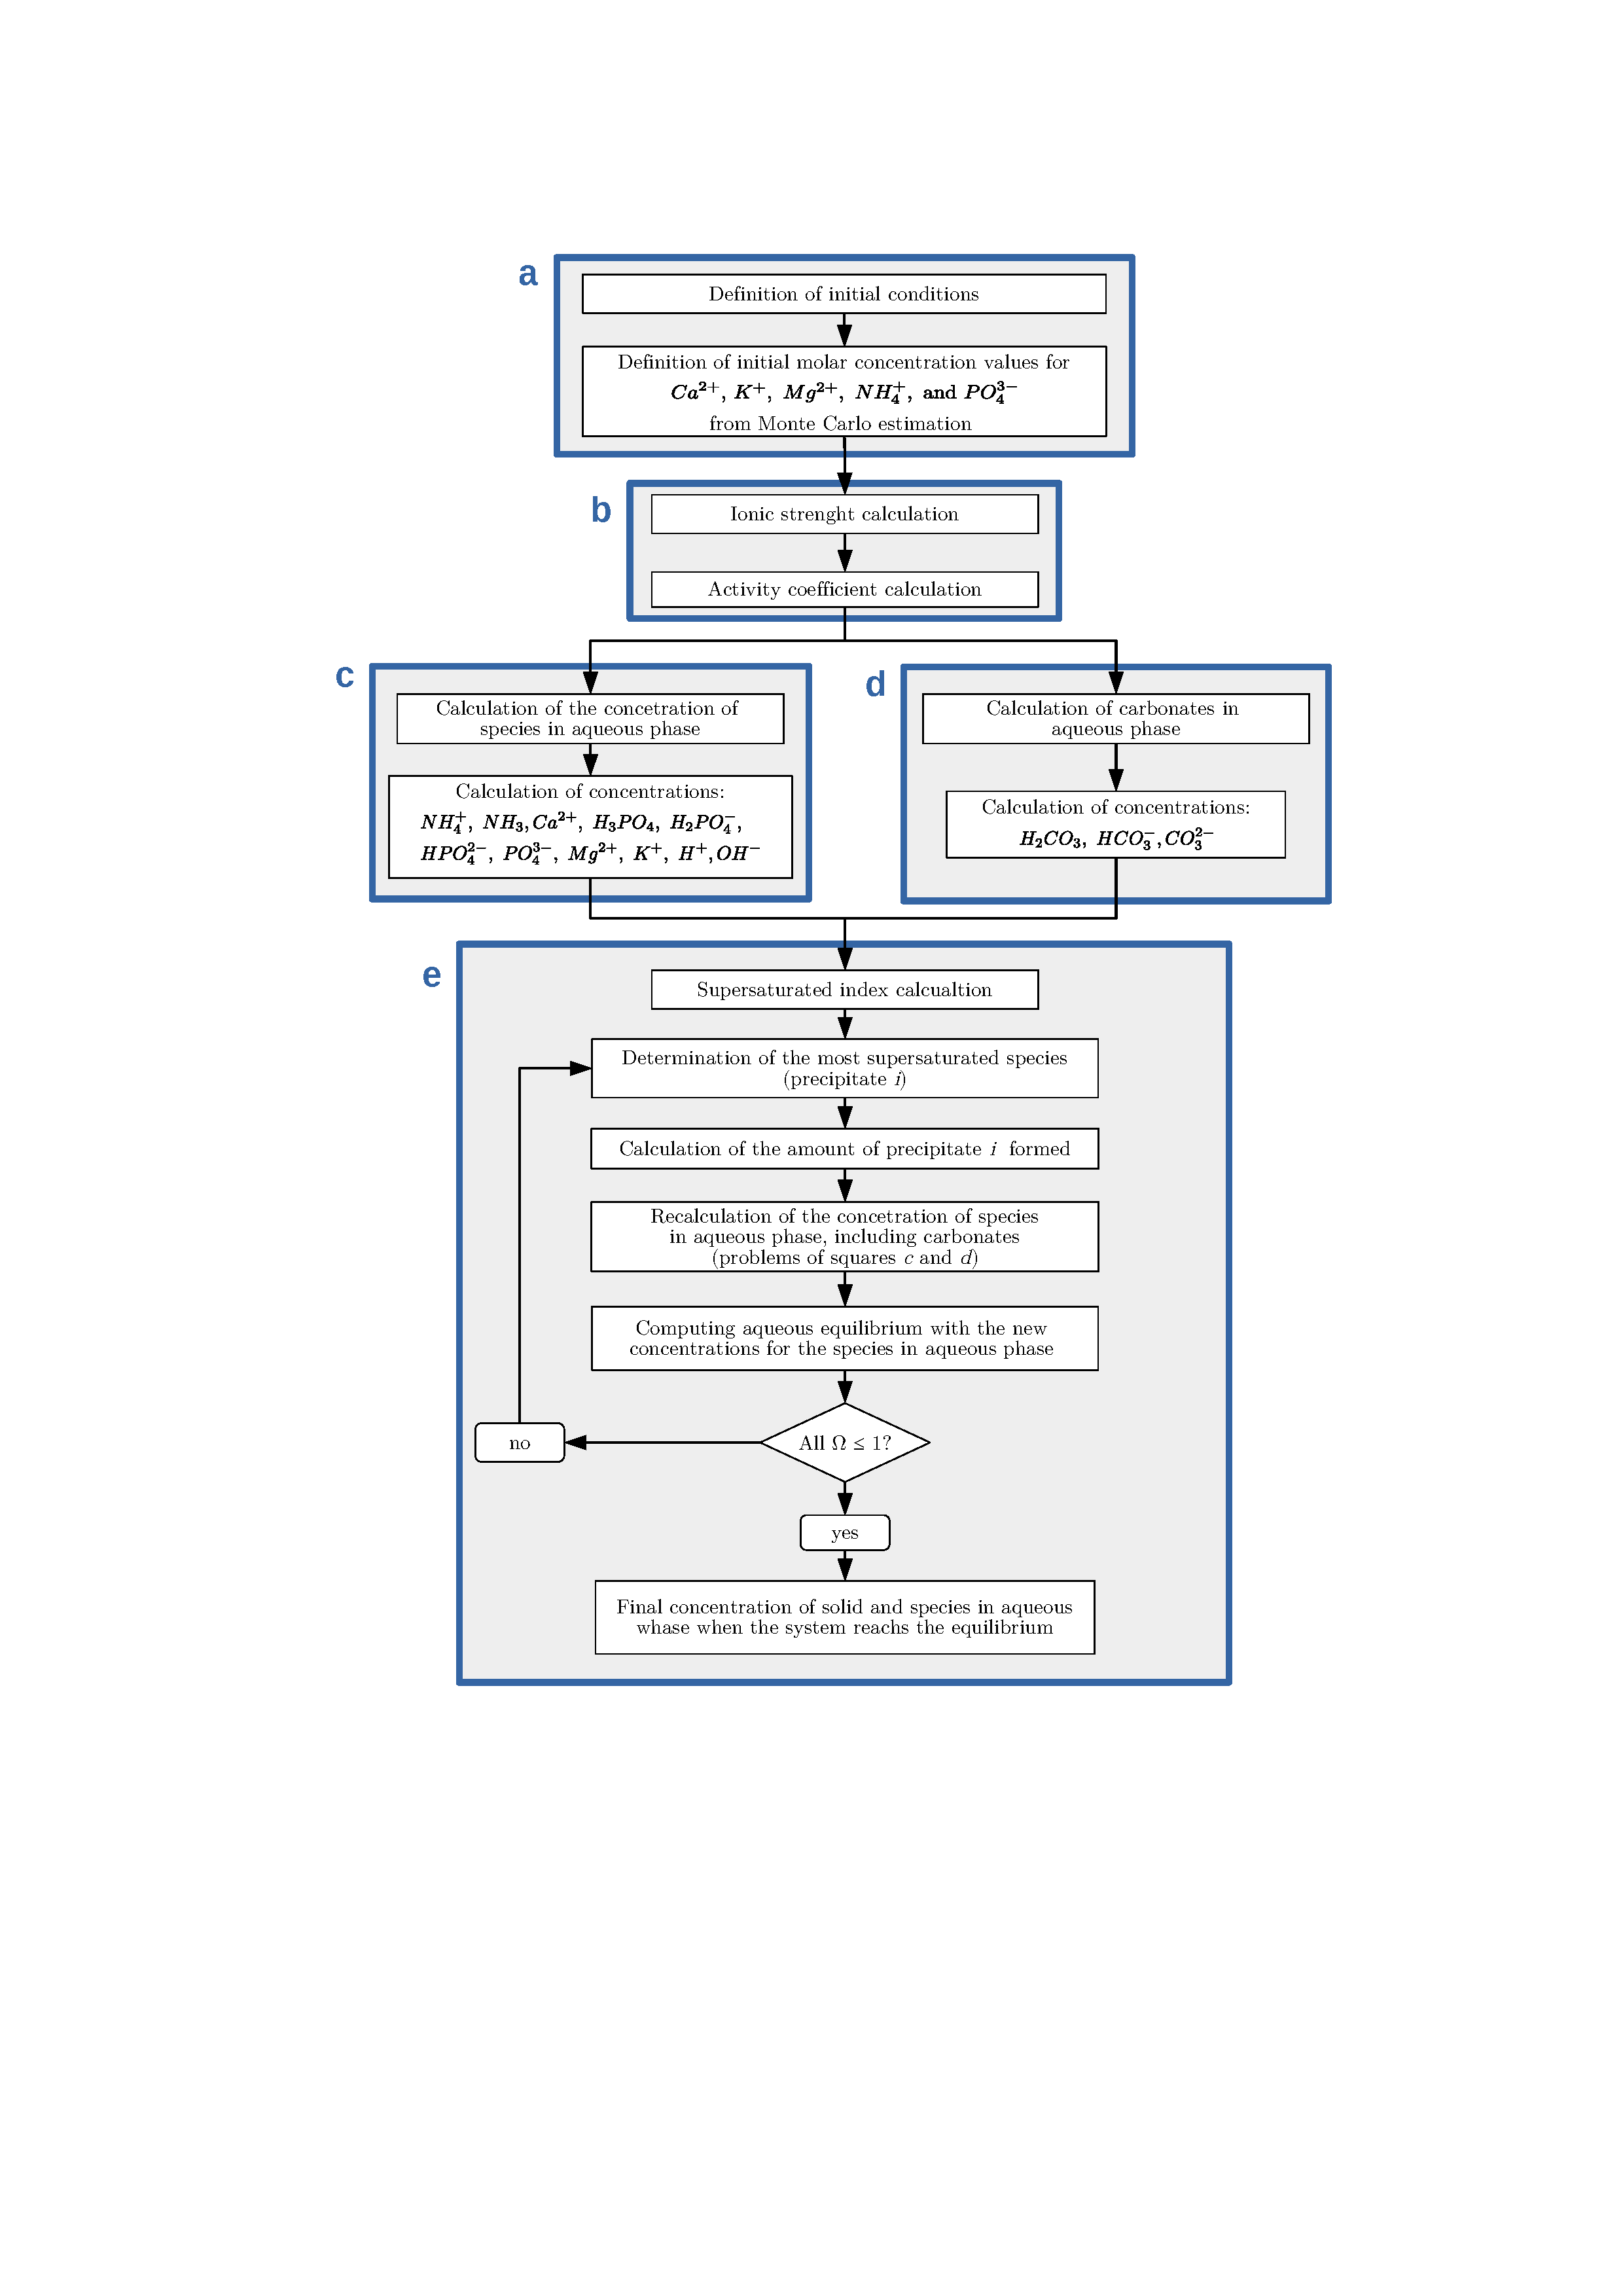
\includegraphics[width=\textwidth, trim=6cm 15cm 6cm 6cm, clip]{gfx/Chapter3/algorithm_flowsheet_w_squares_SUPERREDUCED.pdf} 
	\caption{Flowchart of the proposed algorithm to solve the thermodynamic model for the formation of precipitates in cattle organic waste.} \label{fig:alg_flow}
\end{figure}

\subsubsection{Integration of waste composition uncertainty and precipitates formation thermodynamic models}
\begin{figure}[h!]
	\begin{adjustwidth}{}{} 
		\centering
		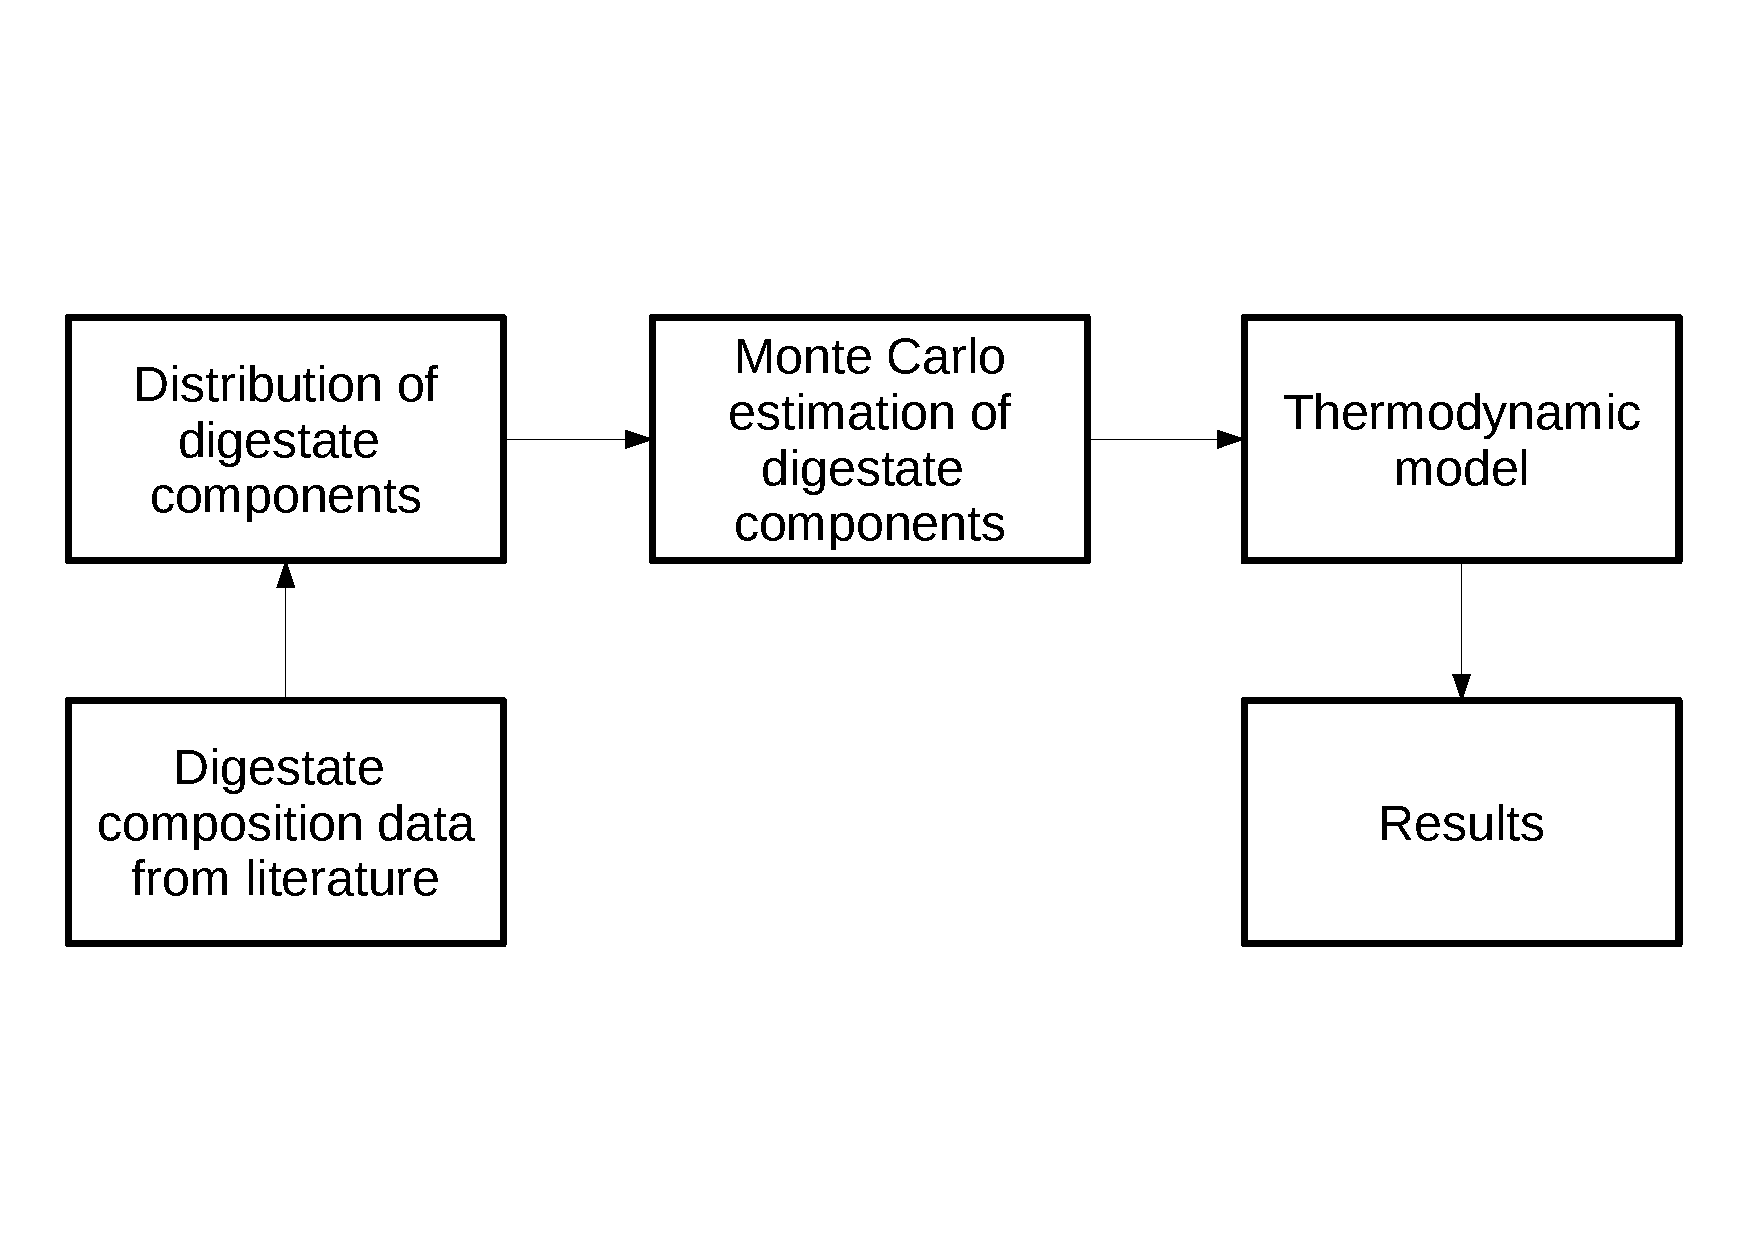
\includegraphics[width=0.85\textwidth, trim=0 4.5cm 0 5cm, clip]{gfx/Chapter3/procedure} 
		\caption{A solution procedure to evaluate the influence of the cattle waste composition variability in the formation of struvite.} \label{fig:procedure_schema}
	\end{adjustwidth}{}
\end{figure}
The evaluation of livestock waste variability in the formation of struvite and other precipitates, consists of 5 steps, as shown in Fig. \ref{fig:procedure_schema}. First, cattle waste composition data are collected from literature. Using these data, probability density distributions for the compounds of cattle leachate are estimated, and they are used in the Monte Carlo model to obtain feasible composition data sets of cattle organic waste. Random points are generated for each chemical compound and species ratios (i.e. N, P, K, Ca, $\text{N-NH}_{4}^{+}:\text{N}_\text{total}$, and $\text{P-PO}_{4}^{3-}:\text{P}_{\text{total}}$). 
Finally, the thermodynamic model is solved for the composition data sets generated, obtaining the precipitated compounds formed.

The thermodynamic model has been implemented in the algebraic modeling language JuMP, embedded in the programming language Julia \citep{DunningHuchetteLubin2017, bezanson2017julia}. The statistical study of cattle waste composition data, the Monte Carlo framework, result analysis, and data visualization were made in Python language \citep{Python, Numpy, Matplotlib, Pandas}.

\subsubsection{Model validation and limitations}
The developed model was validated using the data provided by \citet{Zeng}. Their work was carried out under similar operational conditions to which this work intends to evaluate. In Fig. \ref{fig:validation} experimental and model results are compared. The values at high $\text{Mg}^{2+}$ molar ratio, when the largest supersaturation values are reached and the formation of struvite is close to the maximum allowed by the thermodynamic equilibrium, match the experimental data. However, at lower ratios, differences between results of the thermodynamic model proposed and experimental data can be observed. As the authors of the article indicate, this differences can be due to the presence of many suspended solids which interfere in the struvite formation process. Note that this work is focused on the thermodynamic aspect, without considering other aspects such as chemical kinetics or transport phenomena. The scarcity of data is an impediment to further validate the model.
\begin{figure}[h] 
	\centering
	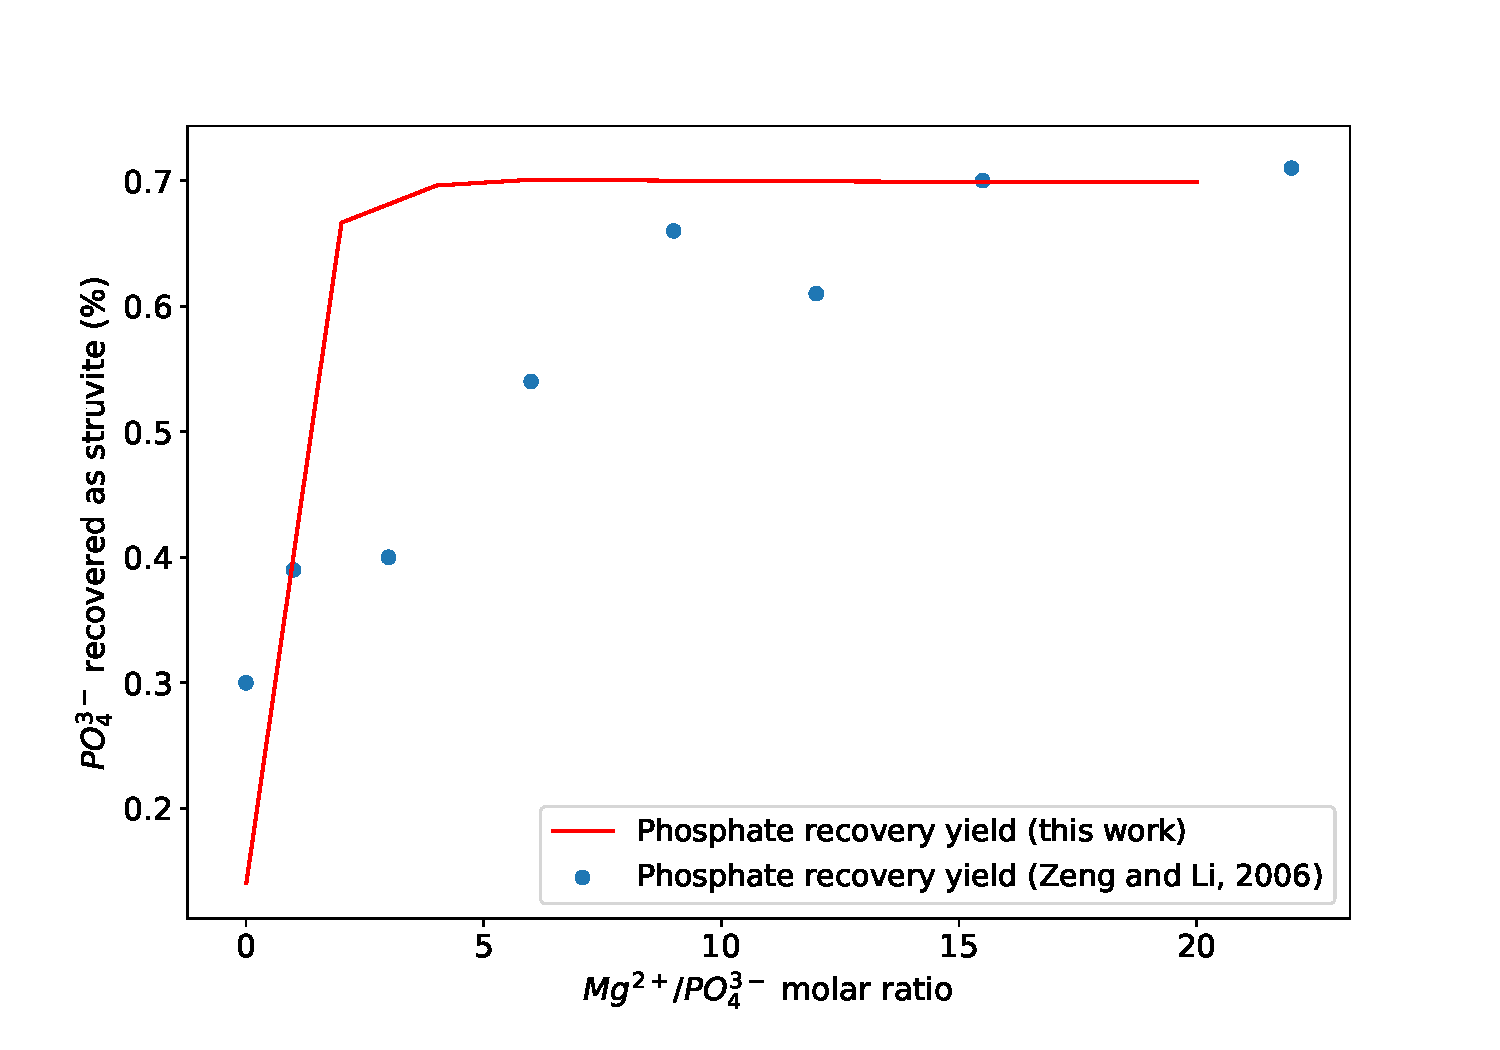
\includegraphics[width=0.9\textwidth, trim=0 0.5cm 0 1.5cm, clip]{gfx/Chapter3/validation.pdf} 
	\caption{Comparison between experimental results reported by \protect\citet{Zeng} and the results provided by the model developed in this work.} \label{fig:validation}
\end{figure}

In addition to the lack of previous studies and data availability to evaluate the effects of kinetics and transport phenomena in the formation precipitates from cattle leachate, another improvement of the proposed model can be achieved by the experimental determination of $pK_{sp}$ values for the potential precipitates formed from cattle leachate. For struvite, the selected $pK_{sp}$ value is taken from the work of \citet{Ohlinger}, as they determined the $pK_{sp}$ value for struvite formation in digestate, a medium with high organic load and dissolved elements like cattle leachate. Otherwise, when $pK_{sp}$ data for cattle waste is unavailable from previous studies, the reported values for water are used. A limitation in the use of the obtained surrogate models is that the formation of struvite and calcium precipitates can only be determined for cattle waste. Although a general formulation for the thermodynamic model is used, and the methodology proposed to include the effect of the uncertainty is not restricted to the use of a specific waste, only cattle leachate has been considered in this study. However, if data on the composition is available, surrogate models to predict the formation of struvite and calcium precipitates from other waste sources can be easily developed.

\section{Results and discussion}
\subsection{Surrogate models to estimate the formation of precipitates from livestock organic waste} \label{results}
The influence of the main controllable parameters for struvite production at industrial scale operation was evaluated: the presence of magnesium and calcium, and the alkalinity. Surrogate models were developed to allow the analytical estimation of precipitates formation. pH value for the struvite precipitation process has been considered as a fixed variable, since there is a wide consensus about a pH value of 9, at which struvite solubility is minimum, is optimal, enhancing the phosphorus and nitrogen conversion to struvite and its eventual precipitation \citep{Tao, Zeng}.

\subsubsection{Influence of magnesium} \label{inf_Mg}
In phosphorus recovery processes through struvite formation, magnesium is usually added to increase the saturation of struvite, enhancing its precipitation. This is especially important for cattle leachate due to the high presence of calcium ions competing with other cations for phosphate anions, and the high ionic strength of livestock leachate, reducing the effective concentration of ions. If the supplementation of magnesium provides enough magnesium ions, struvite will reach higher supersaturation ratio than calcium precipitates, leading the formation of struvite over calcium compounds.
To estimate the performance of struvite precipitation from cattle leachate, the developed thermodynamic model was solved for 50 different composition data sets. The average alkalinity value of the range reported by \citet{Tao} is considered, 8770.5 mg of $\text{CaCO}_{3}$.
The plots showing evolution of precipitates formation in function of the  $\text{Mg}^{2+}/\text{PO}_{4}^{3-}$ molar ratio are collected in the Supplementary Material. 
Analyzing the average fraction of $\text{PO}_{4}$ recovered in form of struvite as a function of the $\text{Mg}^{2+}/\text{PO}_{4}^{3-}$ molar ratio, a tentative value for $\text{Mg}^{2+}/\text{PO}_{4}^{3-}$ molar ratio between 2 and 4 can be set as a compromise effectiveness-cost solution. Higher values result in a considerable consumption of magnesium returning lower improvements in phosphate recovery as struvite.
The surrogate model obtained to evaluate performance of struvite precipitation in function of the magnesium supplied is a Monod type equation, as shown in Eq. \ref{eq:monod_Mg_StrYield}, where $x_{\text{Mg}^{2+}:\text{PO}_{4}^{3-}}$ is referred to the $\text{Mg}^{2+}/\text{PO}_{4}^{3-} \ \text{molar ratio}$.

\begin{align}
& x_{\text{struvite} \left(\text{PO}_{4}^{3-}\right)} = \frac{0.957 \cdot x_{\text{Mg}^{2+}:\text{PO}_{4}^{3-}}}{0.996 + x_{\text{Mg}^{2+}:\text{PO}_{4}^{3-}}} \label{eq:monod_Mg_StrYield} 
\end{align}

The evolution in the formation of calcium precipitates as a function of the $\text{Mg}^{2+}/\text{PO}_{4}^{3-}$ molar ratio was also studied. Hydroxyapatite and calcium carbonate are the only calcium precipitates produced.
Both hydroxyapatite and $\text{CaCO}_{3}$ patterns can be related to the increment of struvite formation along the increase of $\text{Mg}^{2+}/\text{PO}_{4}^{3-}$ molar ratio values, which reduces the presence of phosphate ions, and consequently decreases the supersaturation of hydroxyapatite. Therefore, there are more calcium ions available to form calcium carbonate. 
Surrogate models fit to first order polynomial equations for hydroxyapatite, Eq. \ref{eq:1poly_Mg_HAP}, and for calcium carbonate, Eq. \ref{eq:1poly_Mg_CaCO3}.

\begin{align}
& x_{\text{hydroxyapatite} \left(\text{Ca}^{2+}\right)} = -1.299 \cdot 10^{-2} \cdot x_{\text{Mg}:\text{PO}_{4}^{3-}} + 0.248 \label{eq:1poly_Mg_CaCO3}\\
& x_{\text{CaCO}_{3} \left(\text{Ca}^{2+}\right)} = 1.296 \cdot 10^{-2} \cdot x_{\text{Mg}:\text{PO}_{4}^{3-}} + 0.749 \label{eq:1poly_Mg_HAP} 
\end{align}

\subsubsection{Influence of calcium}
One of the hindrances of cattle leachate for struvite precipitation is the presence of calcium ions competing with other cations for phosphate to form different precipitates.
To study the inhibitory influence of calcium in cattle leachate for struvite precipitation, the thermodynamic model was evaluated for the same 50 different composition data sets used in the previous study along $\text{Ca}^{2+}/\text{PO}_{4}^{3-}$ molar ratio values from 0 to 5. To exclude the influence of magnesium concentration, the study was carried out fixing the $\text{Mg}^{2+}/\text{PO}_{4}^{3-}$ molar ratio at 2.
The plots showing evolution of precipitates formation in function of the $\text{Ca}^{2+}/\text{PO}_{4}^{3-}$ molar ratio are collected in the Supplementary Material. 

The phosphorus as phosphate fraction recovered as struvite exhibits a steep descent at $\text{Ca}^{2+}/\text{PO}_{4}^{3-}$ values between 0 and 2, followed by an asymptotic behavior tending to 0. The dispersion of the values has slight variations along with the evaluated $\text{Mg}^{2+}/\text{PO}_{4}^{3-}$ values.
For hydroxyapatite and calcium carbonate, the higher $\text{Ca}^{2+}/\text{PO}_{4}^{3-}$ value, the greater dispersion for the obtained values. This is due to the increase in the supersaturation values for both calcium precipitates because of the presence of a higher number of calcium ions in the leachate.

The surrogate models obtained for struvite and calcium carbonate fit pseudo-sigmoidal equations, Eqs. \ref{eq:sigmoidal_Ca_StrYield} and \ref{eq:sigmoidal_CaCaCO3} respectively; while for hydroxyapatite (HAP) is a second polynomial function, Eq. \ref{eq:sigmoidal_Ca_HAP}. In all cases, $ x_{\text{Ca}^{2+}:\text{PO}_{4}^{3-}}$ is referred to $\text{Ca}^{2+}/\text{PO}_{4}^{3-} \ \text{molar ratio}$.

\begin{align}
&x_{\text{struvite} \left(\text{PO}_{4}^{3-}\right) }= \frac{0.798}{1+\left(x_{\text{Ca}^{2+}:\text{PO}_{4}^{3-}} \cdot 0.576\right)^{2.113}} \label{eq:sigmoidal_Ca_StrYield} \\
\nonumber \\
%\begin{split}
& x_{\text{hydroxyapatite} \left(\text{Ca}^{2+}\right)} = \label{eq:sigmoidal_Ca_HAP} \\
& -4.321 \cdot 10^{-2} \cdot x_{\text{Ca}^{2+}:\text{PO}_{4}^{3-}}^{2} + 0.313 \cdot x_{\text{Ca}^{2+}:\text{PO}_{4}^{3-}} - 3.619 \cdot 10^{-2} \nonumber 
%\end{split}
\\
\nonumber \\
&  x_{\text{CaCO}_{3} \left(\text{Ca}^{2+}\right)} = \frac{1.020}{1+\left(x_{\text{Ca}^{2+}:\text{PO}_{4}^{3-}} \cdot 0.410 \right)^{1.029}} \label{eq:sigmoidal_CaCaCO3}
\end{align}

\subsubsection{Influence of alkalinity}
Alkalinity is a parameter which can be used to control the production of calcium precipitates. When the presence of carbonates is low, the competition between hydroxyapatite and calcium carbonate tends to benefit the first compound because the limited availability of carbonate ions reduces the supersaturation of calcium carbonate. However, the predominance of hydroxyapatite reduces the formation of struvite since both elements compete for phosphate ions. Therefore, the presence of significant amounts of carbonates (performing at alkaline conditions) reduces the formation of hydroxyapatite and promotes the formation of struvite. 

The results for the formation of struvite, hydroxyapatite and calcium carbonate considering the same 50 different composition data sets used in the previous studies  in function of the alkalinity are collected in the Supplementary Material.
It can be observed that the behavior of struvite formation and calcium carbonate are related, with an abrupt change for both elements at alkalinity values between 3,000 and 4,000 mg of $\text{CaCO}_{3}$, reaching plateaus beyond these values. The dispersion of values follow a similar pattern for both struvite and calcium carbonate, being lower at low alkalinity values, and progressively growing until reaching a value of 4,000 mg of $\text{CaCO}_{3}$. Beyond this value, the dispersion of  values remains constant. Hydroxyapatite formation decrease continuously along the alkalinity values, being complementary with the formation of calcium carbonate.

Therefore, struvite formation from livestock leachate can be enhanced inhibiting hydroxyapatite formation by controlling the alkalinity level, increasing the formation of calcium carbonate and reducing the concentration of calcium ions competing for phosphate. 
Pseudo-sigmoidal fits are shown in Eq. \ref{eq:sigmoidal_Alk_StrYield} for $x_{struvite \left(PO_{4}^{3-}\right)}$, Eq. \ref{eq:sigmoidal_Alk_HAP} for the case of hydroxyapatite, and Eq. \ref{eq:sigmoidal_Alk_CaCO3} for calcium carbonate, where $ x_{Alk}$ is referred to $\text{alkalinity} \left( \text{mg } |\text{CaCO}_{3}\right)$.

\begin{align}
& x_{\text{struvite} \left(\text{PO}_{4}^{3-}\right)} = \frac{0.695}{1+\left(x_{\text{Alk}} \cdot 4.229 \cdot 10^{-4}\right)^{-2.638}} \label{eq:sigmoidal_Alk_StrYield} \\
\nonumber \\
& x_{\text{hydroxyapatite} \left(\text{Ca}^{2+}\right)} = \frac{0.260}{1+\left(x_{\text{Alk}} \cdot 6.460 \cdot 10^{-5}\right)^{3.390}} \label{eq:sigmoidal_Alk_HAP} \\
\nonumber \\
& x_{\text{CaCO}_{3} \left(\text{Ca}^{2+}\right)} = \frac{0.847}{1+\left(x_{\text{Alk}} \cdot 4.646 \cdot 10^{-4}\right)^{-1.870}} \label{eq:sigmoidal_Alk_CaCO3}
\end{align}

\subsubsection{Interactions between calcium and magnesium to phosphate ratios}
Interactions between calcium and magnesium to phosphate ratios were evaluated to determine a target operational area for optimal struvite production performance. In Fig. \ref{fig:struvite_precipitation} the formation of struvite as function of $\text{Mg}^{2+}/\text{PO}_{4}^{3-}$ and $\text{Ca}^{2+}/\text{PO}_{4}^{3-}$ molar ratios is shown, where the area with the highest phosphate recovery in form of struvite has been shaded. It can be observed that struvite formation depends strongly on the $\text{Ca}^{2+}/\text{PO}_{4}^{3-}$ molar ratio. For $\text{Ca}^{2+}/\text{PO}_{4}^{3-}$ values less than 3 struvite formation reaches the maximum values, even for low $\text{Mg}^{2+}/\text{PO}_{4}^{3-}$ molar ratio values. For high calcium/phosphate ratios, struvite formation decreases abruptly, obtaining low increases in struvite formation  even for large supplies of magnesium.

\begin{figure}[h!] 
	\begin{adjustwidth}{}{}
		\centering
		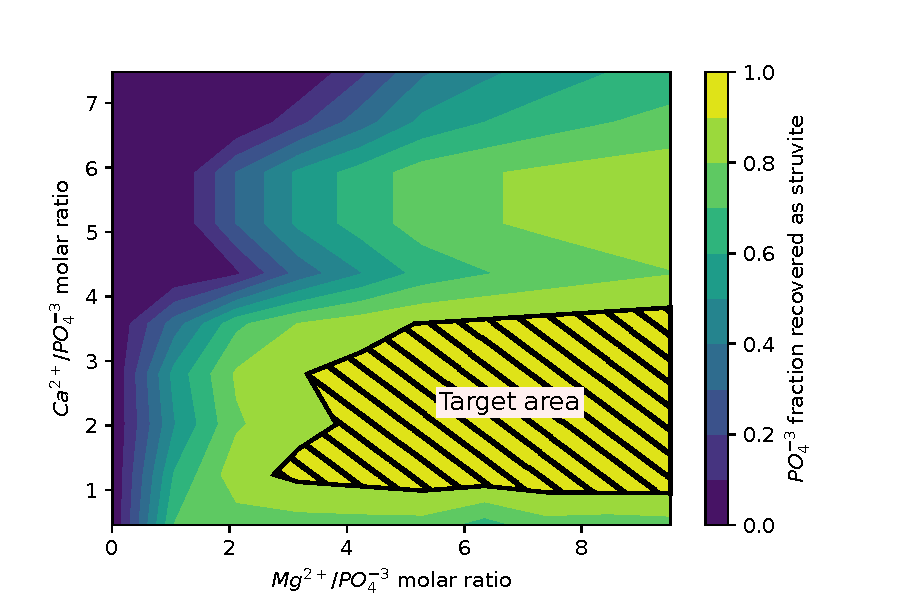
\includegraphics[width=0.6\linewidth, trim=0.5cm 0cm 1cm 1cm, clip]{gfx/Chapter3/Contour_plot_mod.pdf} 
		\caption{Influence of magnesium and calcium in struvite precipitation.} 
		\label{fig:struvite_precipitation}
	\end{adjustwidth}{}
\end{figure}

\subsection{Phosphorus releases from cattle leachate potentially avoided via struvite formation}
Phosphorus pollution of waterbodies, followed by eutrophication and hypoxia scenarios, represents a major environmental problem for the current societies. Considering the United States, the Census of Agriculture reports more than 93 million of cattle heads \citep{2017CensusofAgriculture}, generating an estimated amount of 1,144 million of tons of organic waste per year. The phosphorus contained in the organic waste can be lost as runoff, reaching waterbodies, and polluting the surrounding aquatic ecosystems. Actually, several outstanding cases of eutrophication have taken place in the U.S. in recent times, such as the events occurred in Lake Erie since 1990, and the dead zone in the Gulf of Mexico because of in-excess nutrients discharges collected along the Mississippi River basin. Therefore, nutrient recovery strategies must be implemented to capture phosphorus (and nitrogen) before reaching the waterbodies. Additionally, phosphorus recovery as struvite allows its redistribution to nutrient deficient areas \citep{Martin}.
The surrogate models developed are used to estimate the potential phosphorus emissions avoided in each watershed through phosphorus recovery from cattle leachate as struvite. 

\subsubsection{Balance of phosphorus involved in agricultural activities throughout the U.S. watersheds}
To reach environmental sustainability and reduce the impact over the original ecosystems as much as possible, the releases of phosphorus should be balanced with a coordinated network of phosphorus uptakes. To determine the balance between the releases and uptakes of phosphorus from the agricultural sector, the TES sustainability metric is computed for each watershed in the U.S., showing the watersheds where the phosphorus releases are unbalanced and impacting the environment, Fig. \ref{fig:TES}. For a total of 2,104 HUC8 watersheds, data is unavailable for 6 watersheds, the phosphorus releases and uptakes are balanced in 1,410 watersheds, and 691 exhibit unbalanced phosphorus releases, representing the 33.12\% of total watersheds. It can be observed a larger concentration of unbalanced watersheds along the Mississippi River basin and around the Lake Erie, areas currently affected by eutrophication issues. 

For studies requiring higher spatial resolution, more accurate values for the TES metric can be stimated through the use of local inventories for phosphorus releases and uptakes. A dataset with the phosphorus releases and uptakes, the phosphorus balance, and the TES metric computed for each watershed are available in the Supplementary Material. A dataset with the phosphorus releases and uptakes, the phosphorus balance, and the TES metric computed for each watershed are available in the Supplementary Material.

\begin{figure}[h!] 
	\begin{adjustwidth}{}{}
		\centering
		\includegraphics[width=\linewidth]{gfx/Chapter3/TES_mod.png} 
		\caption{Techno-ecological synergy (TES) metric values for HUC8 watersheds. Red indicates watersheds with unbalanced agricultural phosphorus releases, and blue indicates watersheds with balanced agricultural phosphorus releases. White indicates watersheds with not available data.} 
		\label{fig:TES}
	\end{adjustwidth}{}
\end{figure}

\subsubsection{Phosphorus recovered from cattle leachate through struvite precipitation}
\begin{sidewaysfigure}
	\begin{subfigure}[t]{0.49\textheight}
		\includegraphics[width=\textwidth, trim=55cm 30cm 0cm 0cm, clip]{gfx/Chapter3/scenario1.png}
		\caption{Scenario 1}
		\label{fig:scenario1}
	\end{subfigure}
	%	\quad
	\begin{subfigure}[t]{0.49\textheight}
		\includegraphics[width=\textwidth, trim=55cm 30cm 0cm 0cm, clip]{gfx/Chapter3/scenario2.png} 
		\caption{Scenario 2}
		\label{fig:scenario2}
	\end{subfigure}
	\\
	\begin{subfigure}[t]{0.49\textheight}
		\includegraphics[width=\textwidth, trim=55cm 30cm 0cm 0cm, clip]{gfx/Chapter3/scenario3.png}
		\caption{Scenario 3}
		\label{fig:scenario3}
	\end{subfigure}
	%	\quad
	\begin{subfigure}[t]{0.49\textheight}
		\includegraphics[width=\textwidth, trim=55cm 30cm 0cm 0cm, clip]{gfx/Chapter3/scenario4.png}
		\caption{Scenario 4}
		\label{fig:scenario4}
	\end{subfigure}
	
	\caption{Phosphorus releases avoided through struvite production for the different scenarios considered. Darker colors represent larger phosphorus recovery}
	\label{fig:plot_scenarios}
\end{sidewaysfigure}

Since the scope of the surrogate models developed is limited to the treatment of cattle leachate, only P releases from cattle organic waste will be considered for recovery. Additionally, as it is mentioned in the description of the model, only the phosphate fraction of phosphorus can be recovered through struvite precipitation. Data provided by IPNI NuGIS \citep{NuGIS} report total manure generated, but do not report the breakdown of manure generated by different livestock sources. Therefore, the inventory of cattle for each HUC6 watershed reported by the U.S. Census of Agriculture is used \citep{2017CensusofAgriculture}. To keep spatial consistency between data, the inventory of cattle was aggregated from HUC6 to HUC8 watershed level scaling by the fraction of area represented by each HUC8 basin over the total HUC6 area. The breakdown of cattle types in the U.S. Census of Agriculture is not available at watershed level, but it is available at state level. Therefore, the number of cattle heads is weighted by the fraction of milk and beef animals in the corresponding state. finally, the animals number for each type of cattle is calculated using the normalization values provided by Kellog et al. (2010) \citep{Kellog2000}. If the watershed is shared among several states, the average of the represented states is considered.

Since the supply of magnesium is the easiest controllable variable in the struvite precipitation process, the scenarios evaluated to determine the phosphorus emissions avoided through struvite precipitation were defined through the use of different amounts of magnesium using the surrogate model shown in Eq. \ref{eq:monod_Mg_StrYield}. The different supplies of magnesium have a direct influence on the economy of the process, being one of the highest operating costs items. A summary of the scenarios evaluated and the results obtained is presented in Table \ref{table:scenarios}. The fraction of phosphorus releases avoided is computed over the total phosphorus releases from agricultural activities, including manure releases and fertilizer application, as described in Section \ref{Preleases}. 

\begin{table}[h]
	\centering
	\caption{Scenarios considered and results for cattle leachate phosphorus recovery} \label{table:scenarios}
	\resizebox{0.8\columnwidth}{!}{
	\begin{tabular}{@{}ccccc@{}}
		\toprule
		Scenario                                                                                           & 1       & 2       & 3       & 4       \\ \midrule
		$\text{Mg}^{2+}/\text{PO}_{4}^{3-}$ molar ratio                             & 1       & 2       & 4       & 6       \\
		\begin{tabular}[c]{@{}c@{}}Total P releases avoided\\ (total watersheds) (tons)\end{tabular}       & 422,104 & 562,430 & 674,556 & 722,573 \\
		\begin{tabular}[c]{@{}c@{}}Average P releases avoided\\  (total watersheds) (\%)\end{tabular}      & 22.63   & 30.16   & 36.17   & 38.75   \\
		\begin{tabular}[c]{@{}c@{}}Average P releases avoided\\  (unbalanced watersheds) (\%)\end{tabular} & 18.07   & 24.08   & 28.88   & 30.94   \\
		$\text{kg Mg} / \text{kg P}_{\text{recovered}}$  
		& 2.68    & 4.02    & 6.71    & 9.40    \\ \bottomrule
	\end{tabular}
	}
\end{table}

%\begin{tabular}[c]{@{}c@{}}$\text{Mg}^{2+}/\text{PO}_{4}^{3-}$ \\ molar ratio\end{tabular} 

The results for each scenario considered at watershed scale are shown in Fig. \ref{fig:plot_scenarios}, where darker colors represent larger phosphorus releases avoided. It can be observed that struvite production can contribute to reducing phosphorus emissions around Lake Erie and the Great Lakes region, one of the most severely affected areas by eutrophication problems. Additionally, other areas where the phosphorus emissions avoided are especially significant are the upper basin of the Mississippi River, and the basins located in the south-central region of the United States, such as the areas of some tributaries rivers to the Mississippi River basin, the Rio Grande river and the Colorado River basin. At national level, struvite production can contribute to reduce the agricultural phosphorus releases by 22\% for most conservative case where the lowest amount of magnesium is added. The phosphorus fraction recovered raises until a 30\% and 36\% when the amount of magnesium added is multiplied by 2 and by 4 respectively. However, for the scenario 4 the increase in the supply of magnesium only increases the phosphorus recovered in 2 percentual points compared with the previous scenario. Therefore, the implementation of struvite production processes for phosphorus recovering in cattle facilities can contribute significantly to the reduction in the phosphorus emissions from agricultural operations, reducing the runoffs to waterbodies and mitigating the nutrient pollution of the aquatic ecosystems. However, when only unbalance watersheds are  considered, the average fraction of phosphorus releases avoided decreases, suggesting that, from a global overview, the phosphorus releases due to fertilizers play a major role in these watersheds than when balance and unbalance watersheds are evaluated altogether. Data at watershed level are collected in the Supplementary Material.

Therefore, the phosphorus recovered from livestock facilities have a significant impact in the reduction of phosphorus releases to the environment. However, to achieve a successful implementation of nutrient management strategies, coordinated network management efforts to mitigate nutrient pollution of aquatic systems including point and non-point sources, should be performed for optimizing nutrient management programs that minimize the capital and operating costs while maximizing the environmental benefits. Proposals for the development of coordinated management systems for organic wastes have been presented by \citet{Sharara}, \citet{Sampat3}, and \citet{hu_logistics_2019}.

\section{Conclusions}
To estimate the potential phosphorus releases avoided through struvite precipitation from cattle waste, a thermodynamic framework has been developed to evaluate struvite production from cattle organic waste as a technology for nutrient management and recovery. A set of practical numerical correlations is developed to help predict the struvite recovery. Cattle waste treatment and nutrient recovery through struvite formation is a feasible process from a thermodynamic perspective, reaching phosphate recovery efficiencies up to 80\% with the addition of considerable amounts of magnesium. Additionally, the results show that alkaline conditions can control the calcium ions when their presence in the medium is high and these can interfere in the formation of struvite by precipitating the calcium ions as calcium carbonate, and enhancing the recovery of phosphate as struvite. However, the variability in the organic waste composition is an important parameter that has a high impact on the efficiency of the process. Therefore, an individual composition analysis of the treated cattle waste should be the ideal procedure to achieve the optimal performance of the process by adjusting the operating conditions, particularly the amount of magnesium added and the alkalinity of the medium. Nevertheless, there are opportunities for improving the proposed model by the experimental determination of $pK_{sp}$ values for all potential precipitates from cattle leachate, and by including the effects from kinetics and transport phenomena. 

The techno-ecological synergy sustainability metric (TES) is a useful tool for visualizing the spatial distribution of environmental problems, making it possible to determine what areas are  more sensible to nutrient pollution, and allowing an adequate distribution of efforts to mitigate phosphorus releases and achieved better nutrient management practices. In the U.S., struvite production has large potential for reducing the phosphorus losses from livestock facilities, avoiding between the 22\% and the 36\% of the phosphorus releases from the agricultural sector at national level, reducing the phosphorus runoff and mitigating the nutrient pollution of waterbodies. In addition, it can be observed how struvite production can significantly contribute to reducing phosphorus emissions around Lake Erie and the Great Lakes region, some of the most severely affected areas by eutrophication problems. It should be remarked that the production of struvite from cattle leachate allows the redistribution of phosphorus to nutrient deficient areas reducing the phosphorus runoff to waterbodies and mitigating the nutrient pollution of aquatic ecosystems. However, future research is needed to consider temporal aspects, transportation logistics, and coordinated management strategies for achieving global solutions to global problems. 

%\newpage

\section*{Nomenclature}
\addcontentsline{toc}{section}{Nomenclature}

\vspace{-0.8cm}
\begingroup     
\let\clearpage\relax
%
\newglossaryentry{Ch3var1}{type=VarCh3,name={$A$},description={parameter of the Debye-H\"{u}ckel relationship}}
\newglossaryentry{Ch3var2}{type=VarCh3,name={$E_{x}$},description={emissions of component $x$}}
\newglossaryentry{Ch3var3}{type=VarCh3,name={$EC$},description={electrical conductivity $\left(\frac{\mu \text{S}}{\text{cm}}\right)$}}
\newglossaryentry{Ch3var4}{type=VarCh3,name={$I$},description={ionic strength (M)}}
\newglossaryentry{Ch3var5}{type=VarCh3,name={$K$},description={thermodynamic equilibrium constant}}
\newglossaryentry{Ch3var6}{type=VarCh3,name={$K_{sp}$},description={solubility product}}
\newglossaryentry{Ch3var7}{type=VarCh3,name={$M$},description={equal to $e^{\mu}$}}
\newglossaryentry{Ch3var8}{type=VarCh3,name={$m$},description={stoichiometric coefficient}}
\newglossaryentry{Ch3var9}{type=VarCh3,name={$n$},description={stoichiometric coefficient}}
\newglossaryentry{Ch3var10}{type=VarCh3,name={$T$},description={temperature (K)}}
\newglossaryentry{Ch3var11}{type=VarCh3,name={$U_{x}$},description={uptakes of component $x$}}
\newglossaryentry{Ch3var12}{type=VarCh3,name={$V_{x}$},description={techno-ecological synergy sustainability metric for component $x$}}
\newglossaryentry{Ch3var13}{type=VarCh3,name={$x_{Alk}$},description={alkalinity $\left( \text{mg } CaCO_{3}\right)$}}
\newglossaryentry{Ch3var14}{type=VarCh3,name={$x_{CaCO_{3}}$},description={fraction of calcium recovered as calcium carbonate}}
\newglossaryentry{Ch3var15}{type=VarCh3,name={$x_{Ca^{2+}:PO_{4}^{3-}}$},description={$Ca^{2+}/PO_{4}^{3-}$ molar ratio}}
\newglossaryentry{Ch3var16}{type=VarCh3,name={$x_{hydroxyapatite \left(Ca^{2+}\right)}$},description={fraction of calcium recovered as hydroxyapatite}}
\newglossaryentry{Ch3var17}{type=VarCh3,name={$x_{Mg^{2+}:PO_{4}^{3-}}$},description={$Mg^{2+}/PO_{4}^{3-}$ molar ratio}}
\newglossaryentry{Ch3var18}{type=VarCh3,name={$x_{struvite \left(PO_{4}^{3-}\right)}$},description={fraction of phosphorus as phosphate recovered as struvite}}
\newglossaryentry{Ch3var19}{type=VarCh3,name={$z_{x}$},description={integer charge of ion $x$}}
\newglossaryentry{Ch3var20}{type=VarCh3,name={$\gamma$},description={displacement parameter}}
\newglossaryentry{Ch3var21}{type=VarCh3,name={$\gamma_{x}$},description={activity coefficient for a element $x$}}
\newglossaryentry{Ch3var22}{type=VarCh3,name={$\mu$},description={mean of the distribution}}
\newglossaryentry{Ch3var23}{type=VarCh3,name={$\sigma$},description={standard deviation}}
\newglossaryentry{Ch3var24}{type=VarCh3,name={$\sigma^2$},description={variance}}
\newglossaryentry{Ch3var25}{type=VarCh3,name={$\Omega$},description={supersaturation ratio}}
%
\newglossaryentry{Ch3acro1}{type=AcroCh3,name={AAPFCO},description={Association of American Plant Food Control Officials}}
\newglossaryentry{Ch3acro2}{type=AcroCh3,name={CAFO},description={Concentrated Animal Feeding Operation}}
\newglossaryentry{Ch3acro3}{type=AcroCh3,name={HAB},description={Harmful Algal Bloom}}
\newglossaryentry{Ch3acro4}{type=AcroCh3,name={HUC},description={Hydrologic Unit Code}}
\newglossaryentry{Ch3acro5}{type=AcroCh3,name={KDE},description={Kernel Density Estimation}}
\newglossaryentry{Ch3acro6}{type=AcroCh3,name={USDA},description={United States Department of Agriculture}}
\newglossaryentry{Ch3acro6}{type=AcroCh3,name={USEPA},description={United States Environmental Protection Agency}}
\newglossaryentry{Ch3acro6}{type=AcroCh3,name={USGS},description={United States Geological Survey}}

%
\glsaddall
%**************************************************************
%This is for horizontal spacing between acronym and description
\setlength\LTleft{0pt}
\setlength\LTright{0pt}
\setlength\glsdescwidth{0.8\hsize}
%**************************************************************
%**************************************************************
%This is for vertical spacing between title and entries
\renewcommand*{\glossarypreamble}{\vspace{-0.8cm}}
%**************************************************************
\printglossary[type=VarCh3, style=long]
\vspace{10pt}
\printglossary[type=AcroCh3, style=long]
%\printglossaries
\endgroup


\section*{Acknowledgments} \label{section:Ch3Acknowledgments}
\addcontentsline{toc}{section}{Acknowledgments}
We acknowledge funding from the Junta de Castilla y Le\'{o}n, Spain, under grant SA026G18 and grant EDU/556/2019, and by an appointment for E. Mart\'{i}n-Hern\'{a}ndez to the Research Participation Program for the Office of Research and Development, U.S. EPA, administered by the Oak Ridge Institute for Science and Education. 

\textbf{Disclaimer:} The views expressed in this article are those of the authors and do not necessarily reflect the views or policies of the U.S. EPA. Mention of trade names, products, or services does not convey, and should not be interpreted as conveying, official U.S. EPA approval, endorsement, or recommendation.

\section*{Bibliography}
\addcontentsline{toc}{section}{Bibliography}

\printbibliography[heading=none]
\end{refsection}